\chapter{Plataforma de desarrollo}
\label{cap:capitulo4}
 
Con los objetivos del proyecto definidos, en este capítulo se abordarán las distintas plataformas de desarrollo, tanto \textit{hardware} como \textit{software}, que han facilitado el logro de esos objetivos.

\section{Hardware}
\label{sec:hardware}

Este apartado recoge la descripción de los componentes \textit{hardware} utilizados en este proyecto, para los cuales se ha buscado priorizar la reducción de costes en cada elección y utilizar aquellos elementos a los que se tenía acceso a la hora del desarrollo del proyecto o de los que se disponía a la hora de elaborarlo.

\subsection{Cámara Logitech C270 HD}
\label{subsec:logiC270HD}

Esta cámara web (Figura \ref{fig:logiC270HD}) de dimensiones 72,91 x 31,91 x 66,64 mm, corrige la iluminación de manera automática, produciendo colores reales y naturales y ajustándose a las condiciones de iluminación del entorno, lo que facilita la detección de fresas. Ofrece una resolución HD 720p, proporcionando imágenes claras y nítidas a una velocidad de 30 fotogramas por segundo (fps) con una lente que cuenta con enfoque fijo y un campo visual diagonal (dFoV) de 55 grados. Su coste aproximado es, en la página oficial, de 44€, aunque en otras empresas destacadas en el sector de la electrónica y la tecnología en España puede encontrarse por, aproximadamente, 25€.

\begin{figure} [H]
    \begin{center}
      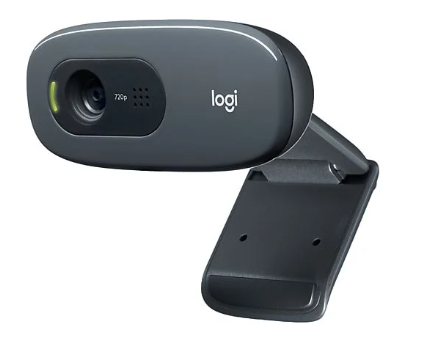
\includegraphics[width=7cm]{figs/logi C270.png}
    \end{center}
    \caption{Cámara Logitech C270 HD$^{\ref{note:enlace16}}$}
    \label{fig:logiC270HD}
\end{figure}

\setcounter{footnote}{16}
\footnotetext[\value{footnote}]{\url{https://www.logitech.com/es-es/products/webcams/c270-hd-webcam.960-001063.html?srsltid=AfmBOor4HptUTcGrxE-4SZxKR-ARw-ykNeagHSEzXUvTlXkx8qLfY4lG}\label{note:enlace16}}

\subsection{Soporte de brazo articulado}
\label{subsec:soporte_camara}

Para poder ubicar la cámara en una posición fija que permitiese visualizar las fresas, se utilizó un soporte de brazo articulado, como el representado en la Figura \ref{fig:soporte_camara}, cuya parte fija en la parte inferior se ancla a la mesa. Este soporte articulado, tiene un ajuste de 360 grados, con su extremo más largo de 75 cm, mientras que la carga máxima que permite es de 560 gramos cuando se coloca de manera horizontal, siendo el precio de este soprte 22,98€.

\begin{figure} [H]
    \begin{center}
      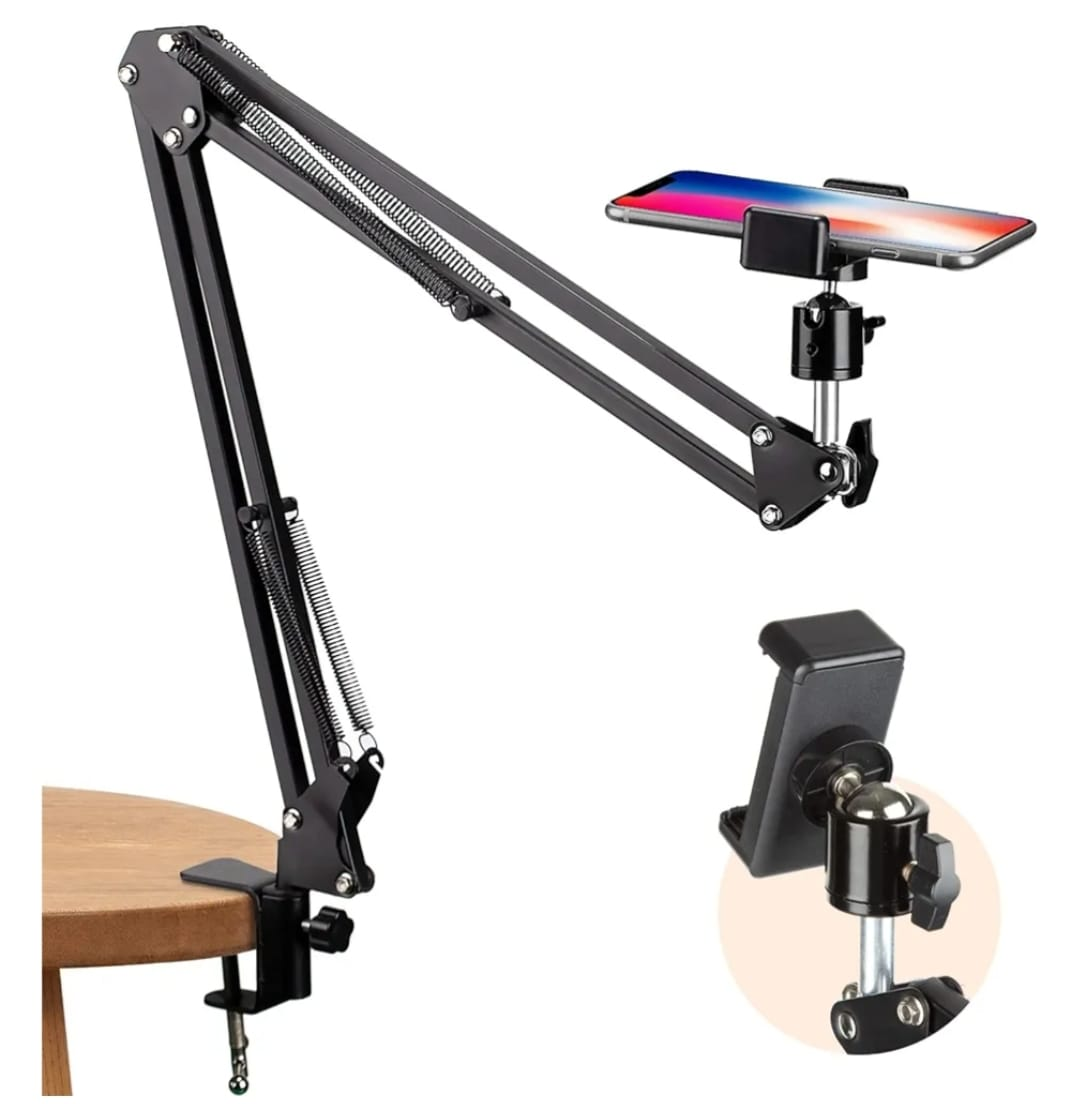
\includegraphics[width=7cm]{figs/Soporte de brazo articulado.jpeg}
    \end{center}
    \caption{Soporte de brazo articulado$^{\ref{note:enlace17}}$}
    \label{fig:soporte_camara}
\end{figure}
 
\setcounter{footnote}{17} 
\footnotetext[\value{footnote}]{\url{https://www.amazon.es/dp/B08JCG4V5S?ref=ppx_pop_mob_ap_share&th=1}\label{note:enlace17}}

\subsection{Ordenador principal}
\label{subsec:ordenador}

El equipo que se ha configurado como entorno de trabajo para este proyecto es el que aparece en la Figura \ref{fig:PC_Lenovo}, sirviendo como base para el desarrollo de la programación y las pruebas de la visión artificial, y utilizándose igualmente como servidor para poder llevar a cabo la comunicación con el brazo robótico mediante el protocolo XML-RPC basado en HTTP, y posteriormente el envío de posiciones detectadas en tiempo real a este. 

\begin{figure} [H]
    \begin{center}
      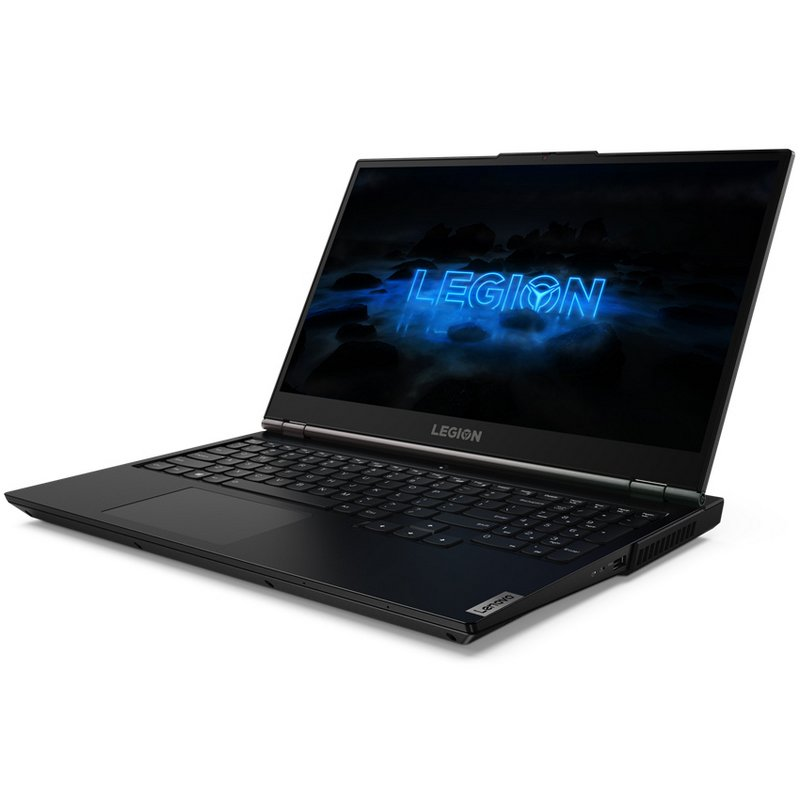
\includegraphics[width=7cm]{figs/Lenovo Legion 5 15imh05.jpg}
    \end{center}
    \caption{Lenovo Legion 5 15IMH05$^{\ref{note:enlace18}}$}
    \label{fig:PC_Lenovo}
\end{figure}

\setcounter{footnote}{18} 
\footnotetext[\value{footnote}]{\url{https://www.pccomponentes.com/lenovo-legion-5-15imh05-intel-core-i7-10750h-16gb-1tb-ssd-gtx-1650-156?srsltid=AfmBOopJpvGSHUyQU696jgG7-6orSKMOEWZe2ZvvYtA0NGtJ9Ms2xJFp}\label{note:enlace18}}

A continuación, en el Cuadro \ref{cuadro:carac_ordena}, se recogen las características técnicas del ordenador utilizado:

\begin{table}[H]
	\begin{center}
		\begin{tabular}{|c|c|}
			\hline
			\textbf{Características} & \textbf{Descripción} \\
			\hline
			\multirow{2}{*}{Pantalla} & \multirow{2}{*}{\shortstack{15,6 pulgadas \\ Full HD (1920x1080)}} \\
			& \\
			\hline
			Procesador (CPU) & Intel Core i7-10750H CPU @ 2.60GHz \\
			\hline
			Memoria RAM & 16 GB \\
			\hline
			Almacenamiento & 1 TB \\
			\hline
			Tarjeta gráfica (GPU) & NVIDIA GeForce GTX 1650 Ti Mobile \\
			\hline
			Sistema Operativo & Windows 10 y Ubuntu 22.04.4 LTS \\
			\hline
			Cámara de portátil & HD 720p con tapa de privacidad \\
			\hline
			\multirow{5}{*}{Puertos} & \multirow{5}{*}{\shortstack{4 x USB 3.2 Gen 1 Tipo-A \\ 1 x USB 3.2 Gen 1 Tipo-C \\ 1 x Ethernet (RJ-45) \\ 1 x HDMI 2.0 \\ 1 x combo auriculares/micrófono (3.5 mm)}} \\
			& \\
			& \\
			& \\
			& \\
			\hline
			Conectividad & WiFi 6 802.11ax (2x2), Bluetooth 5.0, Ethernet 100/1000M \\
			\hline
			Batería & 80 Wh \\
			\hline
			Peso & 2,3 kg \\
			\hline
			Dimensiones & 363,06 x 259,61 x 23,57--26,1 mm \\
			\hline
		\end{tabular}
		\caption{Especificaciones técnicas del ordenador usado}
		\label{cuadro:carac_ordena}
	\end{center}
\end{table}





\subsection{Robot de Universal Robots de la gama e-series}
\label{subsec:URe-series}

\section{Software}
\label{sec:software}

\subsection{Ubuntu}
\label{sec:ubuntu}

\subsection{Python}
\label{sec:python}

\subsection{OpenCV}
\label{sec:OpenCV}

\subsection{Anaconda}
\label{sec:Anaconda}

\subsection{YOLOv3}
\label{sec:YOLOv3}

\subsection{PyTorch}
\label{sec:PyTorch}


